\chapter{Technologies}

    \section{Experience API  \guy{Pierre}}

        \subsection{Présentation et objectif}

            Experience API, abrégée \emph{xAPI} et anciennement connue sous le nom de TinCan, est une norme pour la déclaration d’informations relatives à un processus d’apprentissage. Son objectif est de mettre en place une spécification pour la communication entre les plateformes d’apprentissage et le contenu des formations.

            Experience API est une norme assez récente, sa première version datant de 2013. Elle vise à remplacer SCORM, un modèle plus ancien également utilisé pour normaliser les échanges de données dans le milieu du e-learning. SCORM permet notamment de tracer la complétion, le succès et le temps passé sur une activité.

            xAPI offre cependant une plus grande souplesse dans les déclarations d’activités~: elle permet d’\emph{enregistrer des actions faites par une équipe} et non pas un seul apprenant, ou bien des activités annexes qui sortent du cadre de la formation en ligne (par exemple, lire un livre en rapport avec la formation). 

            De plus, SCORM définit un format d’échange spécifiquement pour le Web, ce qui l’empêche de fonctionner avec des technologies plus récentes, comme les applications mobiles et l’Internet des objets. xAPI n’a pas ces limitations car \emph{son fonctionnement est indépendant du système}.

        \subsection{Fonctionnement}

            \def\myitem#1{\item \emph{\enquote{#1}}:\hspace{2mm}}

            Une déclaration, ou \emph{statement}, représente la trace d’une activité d’apprentissage. Ils sont écrits au format \emph{JSON} (\emph{Javascript Object Notation}), qui permet de représenter simplement des objets sous forme de texte. Chaque déclaration doit renseigner au minimum les trois propriétés suivantes :
            \begin{itemize}
                \myitem{actor} la source de l’action, qui peut être un agent (un individu ou un système), ou bien un groupe d’agents;
                \myitem{verb} l’action effectuée par \enquote{actor};
                \myitem{object} l’activité ou agent sur lequel l’action est faite.
            \end{itemize}

            \let\myitem\relax

            Il existe d’autres propriétés optionnelles, comme \enquote{context} qui donne plus d’informations sur le contexte dans lequel s’est déroulée l’activité, ou \enquote{result} qui détaille le résultat de l’activité.

            Voici un exemple de déclaration valide, qui indique que Paul Durand a assisté à une conférence sur le e-learning :

\begin{lstlisting}[language=json, numbers=none]
{
  "actor": "Paul Durand",
  "verb": {
    "id": "http://activitystrea.ms/schema/1.0/attend",
    "display": { 
      "en-US": "attended" 
    }
  },
  "object": "E-learning conference"
}
\end{lstlisting}

            L’exemple ci-dessus montre qu’il est possible de renseigner uniquement du texte pour une propriété, ou de donner davantage de détails, comme c’est le cas ici pour \enquote{verb}. L’ID du verbe est une URI (l’identifiant d’une ressource) qui fait référence au verbe \enquote{attend} défini dans l’Experience API Registry (une base de ressources en ligne qui permet d’éviter aux utilisateur de xAPI d’avoir à définir leurs propres ressources). L’attribut \enquote{display} indique comment afficher le verbe, et il est possible d’y définir un affichage qui dépend de la langue utilisée.

            Les déclarations créées par xAPI sont enregistrés dans une base de données appelée \emph{LRS} (\emph{Learning Record Store}). Lorsque la plateforme d’apprentissage (aussi appelée \emph{LMS}, pour \emph{Learning Management System}) a besoin d’informations sur le déroulement de la formation d’un apprenant, elle effectue une requête vers le LRS.

            Un LRS peut être intégré à un LMS, ou bien exister de façon séparée. L’important est de stocker l’information de façon normalisée, afin qu’elle soit indépendante du LMS, et puisse être interprétée par des agents extérieurs. Cela ouvre de nombreuses possibilités qui n’étaient pas envisageables avec un système de stockage d’informations spécifique à la plateforme d’apprentissage, par exemple le partage d’informations entre différentes plateformes, ou des études regroupant des données de sources diverses.

        \subsection{Intérêt pour E-Yaka}

            Experience API est une norme qui s’impose dans le monde de l’e-learning aujourd’hui. Comme nous l’avons décrit précédemment, elle permet une grande flexibilité d’utilisation.

            Des bibliothèques existent dans différents langages de programmation pour faciliter l’utilisation de xAPI. E-Yaka est programmé en langage PHP, pour lequel existe la bibliothèque TinCanPHP.

            Il semble donc judicieux d’utiliser Experience API dans le cadre de notre projet.


    \section{Graylog  \guy{Clément}}

        \subsection{Présentation}
    
            Graylog est un système d'analyse de logs libre et open-source. Il offre une interface web sous-forme de tableau de bord (\emph{dashboard}), qui repose elle-même sur une API REST. Son architecture extensible et ses interfaces en font un candidat intéressant pour notre projet, cependant Graylog n'est pas autosuffisant: il doit être couplé à outil de collecte de logs, car il réalise seulement l'étape d'analyse.
    

        \subsection{Fonctionnalités}

            \subsubsection{Interfaces}

                \paragraph{Interface web}
                    Le logiciel serveur de Graylog propose une interface web, qui permet de visualiser des données, et de configurer tous les aspects du serveur.
                
                \paragraph{Interface REST}
                    L'interface Web repose entièrement sur une API REST très puissante, qui permettrait par exemple d'automatiser des tâches de maintenance sur le serveur.

            \subsubsection{Présentation des données}
              
                \paragraph{Moteur de recherche}
                    Graylog intègre un moteur de recherche (ElasticSearch), qui permet de formuler des requêtes élaborées et de trouver les entrées de log qui les satisfont.

                \paragraph{Dashboards}
                    Graylog présente une interface en ligne, centrée autours de \emph{dashboards}. Les dashboards de Graylogs sont configurables et permettent par exemple d'afficher le nombre d'entrée de log qui satisfont une certaine requête. La figure \ref{img:graylog-dash} est un exemple de dashboard. 
                    
                    Plusieurs widgets sont disponibles, mais leur configuration est limitée par la précision du langage de requête du moteur de recherche. 
                    De plus, ces dashboards affichent des données sur l'état de l'application \emph{dans son ensemble}. L'état actuel de nos connaissances ne permet pas de dire s'ils pourront directement être utilisés pour l'interface de l'animateur. 
                    
                    \begin{figure}\centering
                        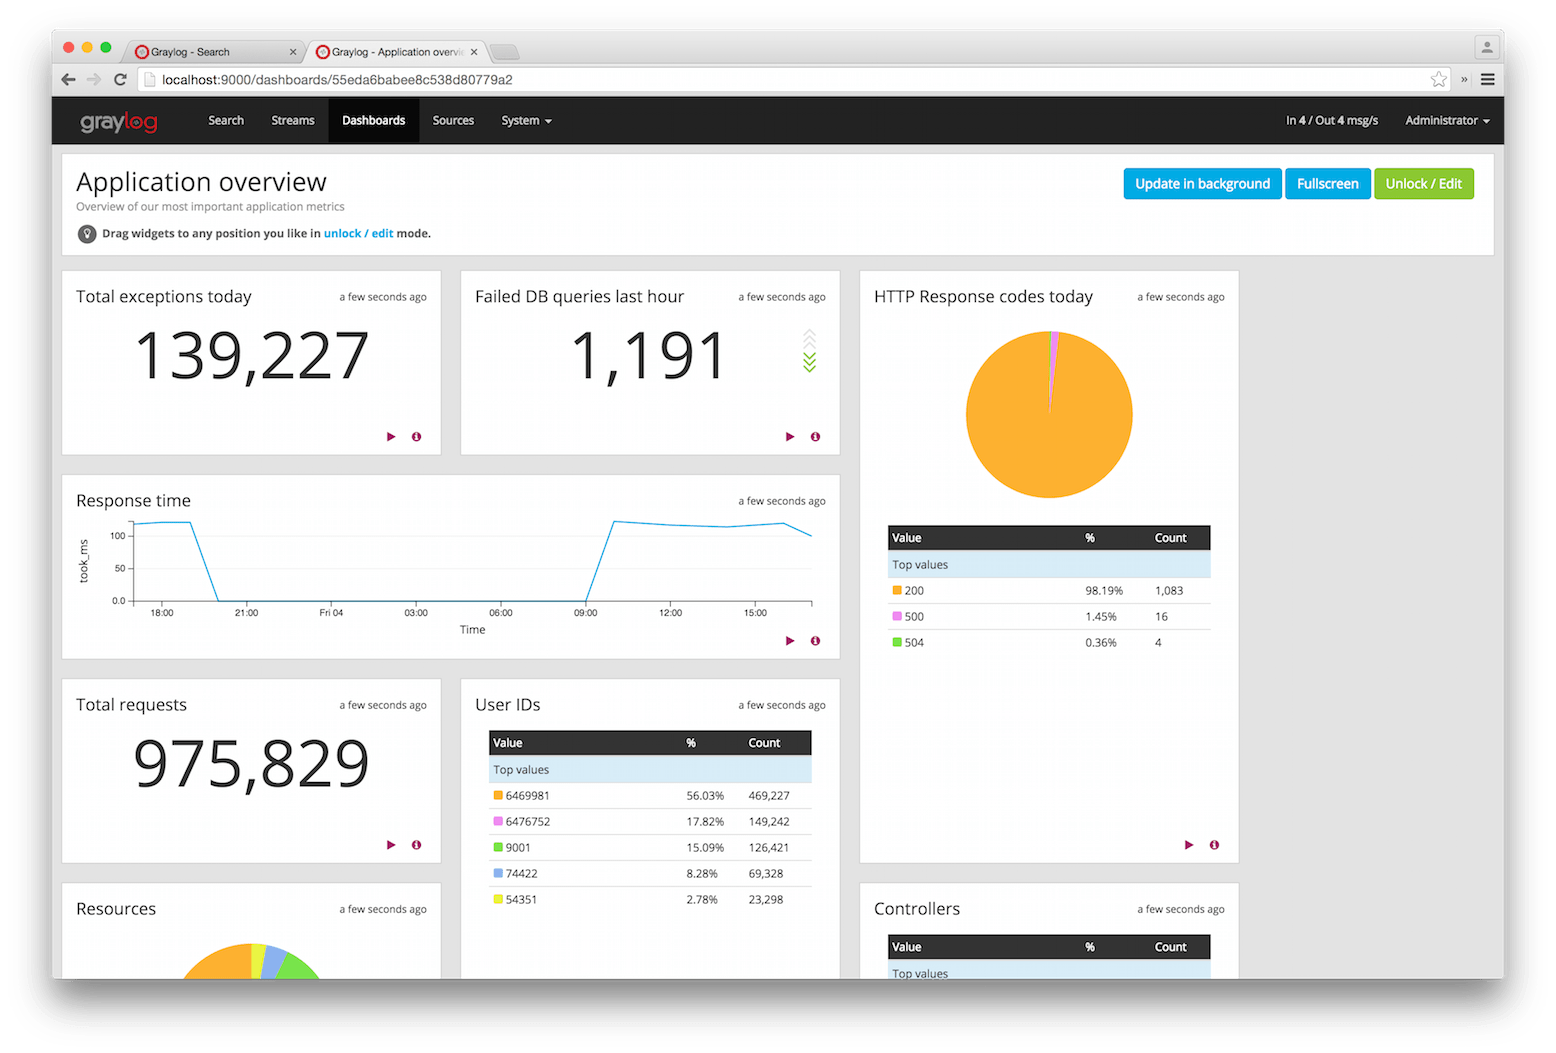
\includegraphics[width=\textwidth]{images/graylog-dash.png}
                        \caption{Exemple de dashboard Graylog}
                        \label{img:graylog-dash}
                    \end{figure}

            \subsubsection{Traitement des données}
                
                Un serveur Graylog reçoit et gère les données d'une application entière. Graylog définit plusieurs abstractions pour les manipuler.
                
                \paragraph{Streams (flots de données)} 
                    Les \emph{streams} Graylog catégorisent et redirigent des messages en temps réel, pendant leur traitement. L'administrateur peut définir des règles pour rediriger les messages qui satisfont une certaine condition dans un stream. Les messages peuvent ensuite être transmis à un autre système, ou à une chaîne de traitement.

                \paragraph{Chaînes de traitement (pipelines)}
                    Une chaîne de traitement définit une séquence d'opérations de filtrage et de traitement, auxquelles les messages en entrée de la pipeline sont soumis. Les instructions de traitement sont écrites en Java, et offrent donc une large marge de manoeuvre.


            \subsubsection{Réception de données}

                \paragraph{GELF}
                    Graylog définit son propre format de message: \emph{GELF}, ou \emph{Graylog Extended Log Format}. Ce format de données est conçu pour pallier aux limitations de \emph{syslog}, un autre format de données qui est le standard \emph{de facto} depuis les années 80. Un message GELF est une chaîne JSON comportant un certain nombre de champs obligatoires. Les messages GELF peuvent être envoyés par UDP, ce qui permet de communiquer facilement avec le serveur de log. Plusieurs librairies pour Symfony 2 supportent l'envoi de messages GELF à un serveur Graylog.

                \paragraph{Autres sources}
                    D'autres types de messages sont supportés, y compris Syslog, ou du texte brut. Il paraît cependant difficile de supporter le format xAPI.

        \subsection{Application à E-Yaka}

            Graylog dispose de nombreuses fonctionnalités attrayantes, y compris des interfaces puissantes, et une grande extensibilité. Cependant l'interface Web du serveur Graylog ne pourra pas être utilisée telle qu'elle, puisqu'il semble difficile de l'intégrer directement dans E-Yaka. Il semble cependant qu'elle faciliterait le travail d'un administrateur.

            L'usage de Graylog impliquerait de plus la sélection d'un outil de collecte de messages pour Symfony. Il en existe plusieurs qui supportent GELF, comme par exemple Monotone (intégré par défaut à Symfony 2), ou FluentD, un outil open-source spécialisé. Ces solutions sont très bien documentées et il semble possible de les implémenter facilement.

    
    \section{Autres technologies}
    
        \subsection{Les cookies, une technologie efficace pour la collecte de logs ?}
        
            Un \emph{cookie} est un fichier de petite taille enregistré sur un ordinateur ou un autre appareil afin de permettre à un site web de reconnaître un utilisateur après sa première visite s'il utilise le même ordinateur et moteur de recherche. Les cookies peuvent avoir plus ou moins \emph{longue mémoire}, pouvant aussi bien conserver des informations sur la dernière visite de l'utilisateur (\enquote{cookie de session}) ou sur de multiples visites précédentes (\enquote{cookie persistant}). D'autres technologies fonctionnent de la même manière, et nous utilisons le mot \enquote{cookie} pour faire référence à tous les fichiers qui collectent des informations de cette façon.
            
            Les cookies ont beaucoup d'usages différents, par exemple enregistrer vos préférences ou encore vous aider à mieux naviguer entre les différentes pages d'un site. Les cookies permettent aussi par exemple d'identifier les contenus les plus populaires d'un site web, et ainsi d'aider les développeurs à améliorer leur site et les services offerts à l'utilisateur.
            
            Il existe plusieurs variétés de cookies et de technologies de traçage, dont par exemple les \emph{Tracking Cookies}, qui permettent d'enregistrer les requêtes HTTP envoyées par une adresse IP (un utilisateur). En voici un exemple simplifié: 
{\small			
\begin{verbatim}            
212.959.120.150 - - [31/Jul/1999:16:58:41 -0400] "GET /last.gif HTTP/1.1"
"http://www.une.org/usnews/home.htm" "Mozilla/4.0" "cookieId=999999"
\end{verbatim}
}            
            
            On peut voir ici que l'utilisateur correspondant à ladresse IP \texttt{212.959.120.150} à demandé à accéder au fichier \texttt{last.gif} sur la page d'accueil du site \texttt{www.une.org}.
            
            Cependant, nous ne pourrons pas utiliser cette technologie pour plusieurs raisons, notamment pour une question juridique, puisque les utilisateurs doivent consentir explicitement à l'utilisation de cookies pour les tracer, ce qui pourrait nous empêcher de connaître leurs activités sur l'application. De plus, cela pose des complications technologiques puisque, les cookies étant par définition stockés sur l'ordinateur de l'utilisateur, ils sont inaccessibles lorsque l'utilisateur est hors ligne.
        
        \subsection{Apache log4php 2}
        
            Presque toutes les grosses applications utilisent leurs propres API de traçage. Les frameworks de logging tels que Log4php sont conçus pour limiter la consommation de ressources nécessaires à la mise en œuvre d'une API de logging.
% * <cl-fournier@live.com> 2017-10-19T15:28:29.273Z:
% 
% Tu peux reformuler cette phrase? C'est pas clair (ex. de quel type de ressource tu parles). Intuitivement j'aurais plutôt dit que ces framework servent à offrir des solutions unifiées non? ou bien à limiter le temps de développement d'une solution spécifique  à l'application, enfin j'en sais pas grand chose
% 
% ^.
% * <cl-fournier@live.com> 2017-10-19T15:28:28.355Z:
%
% ^.
            
            Log4php est un framework open-source proposant une API qui permet aux développeurs d'utiliser et de paramétrer un système de gestion de journaux (logs). Log4php gère plusieurs niveaux de gravités et les messages peuvent être redirigés vers plusieurs flux : un fichier sur disque, le journal des événements de Windows, une connexion TCP/IP, une base de données, etc ...
        
            Log4php utilise trois composants principaux pour assurer l'envoi de messages selon un certain niveau de gravité et contrôler à l'exécution le format et la ou les cibles de destination des messages :

            \begin{itemize}
                \item Category/Logger : ces classes permettent de gérer les messages associés à un niveau de gravité;
                \item Appenders : ils représentent les flux qui vont recevoir les messages de log;
                \item Layouts : ils permettent de formater le contenu des messages de log.

            \end{itemize}

            Ces trois types de composants sont utilisés ensemble pour émettre des messages vers différentes cibles de stockage. Ceci permet au framework de déterminer les messages qui doivent être loggués, la façon de les formater et vers quelle cible les messages seront envoyés.

            La popularité de log4php est largement liée à  ses nombreuses fonctionnalités extensibles et sa fiabilité. Cependant, il est le plus souvent utilisé en tant qu'outil de déboguage et de sécurisation et nous paraît plus difficile à implémenter.
        
        \subsection{BeamPulse : vers l'analyse d'interface}
        
            Il existe d'autres technologies intéressantes afin d'améliorer l'utilisation de l'application E-Yaka. Une  amélioration possible est l'augmentation de l'efficacité de l'interface web à l'aide d'outils tel que BeamPulse. BeamPulse est une solution permettant d'analyser, améliorer et personnaliser votre site web à l'aide de fonctionnalités telles que :
            \begin{itemize}
                \item Des cartes de chaleurs (\emph{heat maps}) : \emph{heat maps} de clic et de défilement pour visualiser les incompréhensions et blocages sur chaque page;
                \item \emph{Session Recording} (\emph{playback}) : Enregistrer et observer le tracé des mouvements de la souris, les défilements, les clics et les temps d'attente sur le site afin de les rejouer devant le développeur;
                \item Personnalisation temps-réel : Modifier le contenu de vos pages ou déclencher automa\-tiquement des interactions ciblées en temps-réel.
            \end{itemize}
            
            Cet objectif d'amélioration de l'interface ne fait pas partis de notre cahier des charges, mais il pourra cependant être envisagé si notre projet se termine en avance, ou encore comme suite du projet.
        